%-------------------------------------------------------------------------------
\chapter{Speciális platformok megjelenése}
%-------------------------------------------------------------------------------
\section{hybrid deep learning}
A ha

\section{nGraph}
A most leírtak alapját az nGraph hivatalos dokumentációja adja\cite{web:ngraph_intro}.
Az nGraph az Intel\registeredlogo által fejlesztett programkönyvtár és egy futtatási környezet/fordító készlet melyet mély tanuló projektekhez.
Legszembetűnőbb tulajdonsága, hogy képes többféle hardver architektúrán futtatni és beépíthető számos keretrendszerbe.
Ezek azok a jellemzők, amiket kerestünk témavezetőmmel, hogy mély tanulást tudjunk végeztetni hatékonyan a \emph{HuSSar-on}. 
Ezen túlmenően a jövőbeli fejlesztések az iparban egyre jelentősebben igényelik, hogy a modern MI rendszerek skálázhatóak legyenek, mert egyrészt a neurális hálók egyre komplexebbé válnak, másrészt az általuk feldolgozott adatok mennyisége is rohamosan növekszik.

Jelenleg két bevett gyakorlat van a mély tanulás felgyorsítására:
\begin{enumerate}
	\item \textbf{Dedikált hardver tervezése a mély tanulással kapcsolatos számításokhoz} -- Sok vállalkozás tervez \emph{Alkalmazásspecifikus integrált áramköröket} (ASIC) neurális hálózatok betanítására és futtatására.
	\item \textbf{Szoftver optimalizáció} -- Programkönyvtárakat tartalmazó fejlesztési keretrendszerek fejlesztése, melyek képesek a hálózatokkal kapcsolatos számításokat több szálon, optimalizáltan futtatni. Az nGraph, mint fordító is egy ilyen megoldás.
\end{enumerate}

\subsection{Motiváció}
A mai legmodernebb szoftveres megoldás mély tanulásra az, ha integrálunk kernel könyvtárakat\footnote{Programkönyvtár, mely neurális hálókkal kapcsolatos elemi, \emph{mag} függvényeket tartalmazzák} mély tanulási keretrendszerekbe.
Ilyen integráció lehet például ha a Tensorflow keretrendszer alatt az Nvidia CuDNN könyvtárát használjuk.
A {kernel könyvtárak} egy adott célarchitektúrára optimalizált kernelekből és egyéb műveleti szintű optimalizálásokból állnak, ezekkel érve el teljesítménynövekedést.
Azonban a kernel könyvtáraknak három fő problémája van:
\begin{enumerate}
	\item Nem biztosítanak gráf szintű optimalizálást
	\item A keretrendszerek integrációja a {kernel könyvtárakkal} nem skálázható
	\item A szükséges lefordított kernel könyvtárak száma növekszik, ahogy új processzorok jelennek meg
\end{enumerate}
Az nGraph fordító megoldás az első két problémára, és a \emph{PlaidML}-el ötvözve kiküszöbölhető a harmadik probléma.
\subsection{Gráf szintű optimalizálás}
Az nGraph dokumentációjában áll egy példa arra vonatkozóan, hogyan lehet, hogy egy mély tanulási keretrendszer integrálva egy {kernel könyvtárral} a számításokat optimálisan végzi, mégis a számítási gráf a csúcsait alkotó műveletek szempontjából mégsem optimális.
\begin{figure}[!ht]
	\centering
	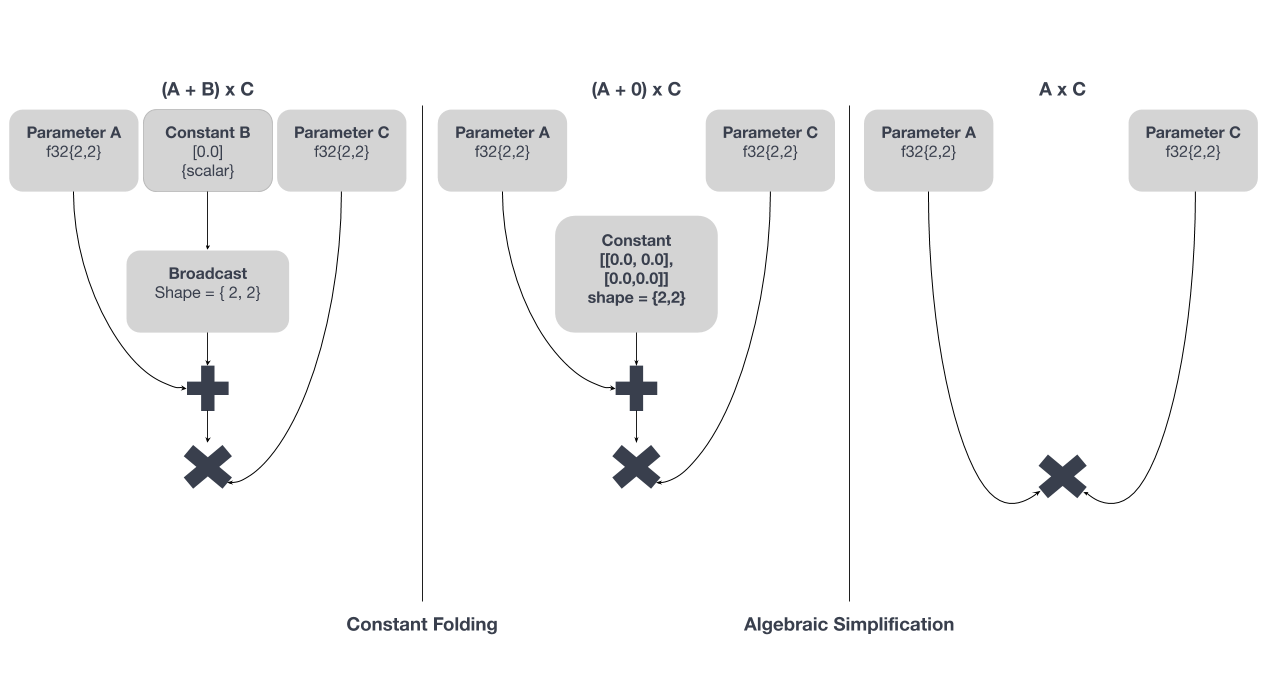
\includegraphics[width=0.9\textwidth]{kernel-problem-1.png}
	\caption{két optimalizálás módszer: konstans összehajtás és algebrai egyszerűsítés a gráfon. \protect \footnotemark}
	\label{fig:grafoptimalizalas}
\end{figure}
\footnotetext{forrás: \cite{web:ngraph_intro}}
A fenti ábra bemutatja, hogyan egyszerűsíthetünk az $A$,$B$ és $C$ tenzorokat feldolgozó, $ (A+B)*C $ tenzorműveletet végrehajtó számítási gráfon.
Fordítási időben megállapítható, hogy $B$ egy skalár konstans, így a \emph{konstans összehajtásnak} nevezett optimalizálás elvégezhető, és a 2 dimenziós vektorrá való kiterjesztés művelete elhagyható (helyette inkább közvetlenül létrehozunk egy $2\times2$ tenzort).
Ebben a példában $B=0$ skalár volt, így a belőle létrejött tenzor egy nullmátrix, így az semleges a kifejezés kiértékelésének szempontjából.
\emph{Algebrai egyszerűsítést} végezve az $ (A+0)*C $ leegyszerűsíthető az $A*C$ kifejezésre, így összesen két csúccsal csökkentettük a gráfunkat.
Ez az optimalizáció tehát a számítási gráf szintjén lett elvégezve.
Így belátható, hogy a mély tanulási keretrendszerbe integrált kernel programkönyvtárak nem optimális futást végeznek, hiába a műveletek szintjén elért optimalizálás. 
\subsection{Skálázható keretrendszer integráció}
Ahogy gyarapodik a mély tanuláshoz használható gyorsítókártya architektúrák és keretrendszerek száma, a meglévő mély tanulást alkalmazó fejlesztési platformok bővítése egyre több munkát igényel és egyre nő a hibák megjelenésének a valószínűsége. Az integráció kapható készen, szakértő fejlesztőcsapatoknak kell implementálnia.
Minden új keretrendszert manuálisan kell integrálni a meglévő hardverek kernel könyvtárával és minden újonnan megjelenő hardvercsalád meghajtó programkönyvtárát be kell integrálni egyesével a meglévő keretrendszerekbe.
Ez a munka önmagában is hatalmasra tud nőni, de egy sok eszközből álló összeállítás nagyon törékeny és költséges a fenntartása.
Az nGraph úgy oldja meg ezt a problémát, hogy ún. \emph{hidakat} alkalmaz, amikkel integrálható valamelyik mély tanulási keretrendszerbe.
A híd megkapja a keretrendszerben megalkotott számítási gráfot vagy ahhoz hasonló struktúrát és átalakítja egy ún. \emph{közbenső reprezentációvá}\footnote{IR: Intermediate Representation}. Ezzel kaptunk egy egységes, platformfüggetlen számítási gráfot, így nem kell egy új programkönyvtárat beintegrálni minden egyes meglévő keretrendszer alá, elegendő csak az, hogy az nGraph-ban, mint programkönyvtárban implementált \emph{primitív műveleteket} támogassa az új programkönyvtár.
\subsection{Növekvő kernel szám}
Egy kernel könyvtár integrálása egyszerre több mély tanulási keretrendszerrel nehéz feladat és egyre komplexebbé válik, ahogy növekszik az optimális teljesítményhez szükséges kernelek száma.
Régen a mély tanulással kapcsolatos kutatások egy kis számú \emph{primitív} számítást használtak, mint a konvolúció, általános mátrixszorzás, stb. Az MI kutatás előrehaladtával és az ipari mély tanuló alkalmazások továbbfejlesztésével, a szükséges kernelek száma (k) exponenciálisan nő.
Ez a szám a processzor architektúrák számán (h), adattípusokon (t), műveleteken (p) és az egyes paraméterek számosságán (p) alapul ($ k = h \times t \times m \times p $).
\begin{table}[!ht]
	\centering
	\begin{tabular}{|c|c|c|c|}
		
		Hardver & Művelet & Adattípus & Paraméterek \\ 
		\hline
		CPU & konvolúció & 16 bites lebegőpontos & NCHW vagy NHWC \\ 
		
		GPU & MatMul & 32 bites lebegőpontos & 2D, 3D és 4D tenzorok \\ 
		
		FPGA & Normalizálás & 8 bites egész &  \dots \\ 
		
		\dots & \dots & \dots & \\
	\end{tabular} 
	\caption{Néhány példa, tényezőnként hányféle esetre kell külön fordítani  kernelt könyvtárt }
	\label{table:kernels}
\end{table}

Ezen probléma megoldásához jön képbe a PlaidML. Ez egy \emph{tenzor fordító}\footnotemark, mely azt célozza, hogy képes legyen neurális hálózatokat tanítani és futtatni bármilyen típusú hardveren. Más szavakkal segíti a magas szintű keretrendszerek (Keras, ONNX, nGraph) integrálni olyan ezsközökkel, melyekhez nincs meg a szükséges támogatás vagy a meglévő szoftverkészlet hozzájuk szigorúan linceszelt.\cite{github:PlaidML}\cite{web:PlaidML}
\footnotetext{Olyan fordító, melynek nyelve arra lett fejlesztve, hogy főleg tenzorműveleteket igénylő számításokat tudjunk hatékonyan programozni}

Az nGraph tehát integrálható a PlaidML-el. Elsősorban az nGraph a platform független IR-rel igyekszik orvolsoni a skálázható backend-el kapcsolatos kihívást. A PlaidML ezt megtámogatja azzal, hogy képes az IR-ből származó gráfokból LLVM, OpenCL, OpenGL, CUDA és Metal kódot generálni melyek a megfelelő hardveren futtathatóak. Így egy magas szintű keretrendszerben írt neurális háló lefordul Intel és AMD processzrokon valamint grafikus processzorokon, az nVidia processzorain, továbbá az Apple cég által feljelsztett eszközökön.

Az nGraph gráf szintű optimalizációját ráadásul kiegészíti automatikusan a PlaidML alacsonyabb szinten, ezzel teljesítmény növekedést érve el.

Összegzésül tehát az nGraph feldarabolja a neurális hálózathoz tartozó számítási gráfot processzor architektúrának megfelelően, majd ezen gráfokat a PlaidML lefordítja a megfelelő kódokra, melyeket aztán a célprocesszorokra lefordítunk és futtatunk.

\section{Myriad X és az Intel Neural Computer Stick 2}

%Motiváció: Valós idejű alkalmazások esetén szükséges az offline számítás -> GPU - lehetséges, de erőforrás igényes(áram és hűtés) és nagy méretű 

%TODO Nincs Befejezve

\section{Google Edge TPU}
Az Intelhez hasonlóan a Google is tervezett célprocesszort és hozzá fejlesztő panelt, mély tanulást alkalmazó projektekhez. A Google Edge TPU-ról és a Coral USB Accelerator-ról a Heartbeat internetes magazinban megjelent cikkben értesültem.\cite{web:GoogleEdge}

Ugyan azt az igényt igyekszik kielégíteni, mint a korábban bemutatott Myriad X processzort és az Intel Neural Compute Stick 2. A valós idejű mély tanuló alkalmazások igénylik az offline módon történő számítást kis fogyasztás mellett.
Az Intel-től eltérően a Google ún. Tensor Processing Unit-ot, egy saját fejlesztésű gyorsítókártyát használ a neurális hálózatokkal kapcsolatos számítások optimalizálására. Ezeket a társprocesszor kártyákat a Google a saját adatközpontjaiban használja főként és elérhetővé teszi őket a \emph{Google Cloud Platform} nevű szolgáltatásán keresztül. Nevéből adódóan a kártya architektúrája lehetővé teszi, hogy  tenzorműveletek tudjanak hatékonyan végrehajtani, utasításkészletük kifejezetten támogatja a neurális hálózatokat. Ilyen művelet a mátrix szorzás, konvolúció és az aktváló függvények alkalmazása az \ref{section:neuralNetworkTheory} alfejezetben tárgyalt módon. 

Az Edge TPU már egy alkalmazásspecifikus integrált áramkör más néven ASIC.
%TODO Nincs Befejezve


\section{Új gyorsítók: Intel Nervana Neural Network Processor}

%TODO Nincs Befejezve